\titledquestion{Théorie des graphes}
Le président des USA, n'ayant pas aimé avoir été corrigé sur son utilisation du mot ``French fries'' par le premier ministre belge,
a décidé de faire passer les taxes sur les produits importés à 60\%.
La Belgique a alors automatiquement riposté avec une taxe équivalente pour ses importations des USA.
Le gouvernement belge vous demande de trouver s'il est possible de payer moins de taxe pour vendre ou acheter des produits avec les USA
en passant par des pays intermédiaires.

\begin{center}
    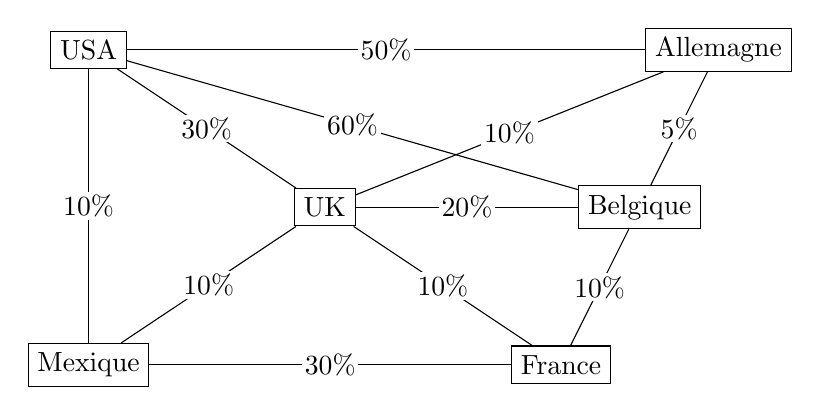
\begin{tikzpicture}[scale=2]
        \node[draw,rectangle] (BE) at (0.5,1) {Belgique};
        \node[draw,rectangle] (FR) at (0,0) {France};
        \node[draw,rectangle] (DE) at (1,2) {Allemagne};
        \node[draw,rectangle] (UK) at (-1.5,1) {UK};
        \node[draw,rectangle] (US) at (-3,2) {USA};
        \node[draw,rectangle] (ME) at (-3,0) {Mexique};

        \path [draw,-,>=stealth] (BE) edge node[midway,fill=white,inner sep=1pt]{10\%} (FR);
        \path [draw,-,>=stealth] (BE) edge node[midway,fill=white,inner sep=1pt]{5\%} (DE);
        \path [draw,-,>=stealth] (FR) edge node[midway,fill=white,inner sep=1pt]{10\%} (UK);
        \path [draw,-,>=stealth] (DE) edge node[midway,fill=white,inner sep=1pt]{10\%} (UK);
        \path [draw,-,>=stealth] (UK) edge node[midway,fill=white,inner sep=1pt]{30\%} (US);
        \path [draw,-,>=stealth] (DE) edge node[midway,fill=white,inner sep=1pt]{50\%} (US);
        \path [draw,-,>=stealth] (UK) edge node[midway,fill=white,inner sep=1pt]{10\%} (ME);
        \path [draw,-,>=stealth] (FR) edge node[midway,fill=white,inner sep=1pt]{30\%} (ME);
        \path [draw,-,>=stealth] (ME) edge node[midway,fill=white,inner sep=1pt]{10\%} (US);
        \path [draw,-,>=stealth] (BE) edge node[midway,fill=white,inner sep=1pt]{20\%} (UK);
        \path [draw,-,>=stealth] (BE) edge node[midway,fill=white,inner sep=1pt]{60\%} (US);
    \end{tikzpicture}
\end{center}

\begin{parts}
    \part Quel serait la meilleure manière de faire, étant donné les taxes bilatérales données ci-dessus.
    \emph{Hint: Combiner deux taxes de 10\% et 20\% correspond à $1.1 \cdot 1.2 = 1.32$.}
\begin{solutionbox}{4cm}
    On a
    $$1.05 \cdot (1.1)^4 < 1.3 \cdot 1.2 < 1.3 \cdot (1.1)^2 < 1.05 \cdot 1.5 < 1.6$$
    donc le plus court chemin est de passer par l'Allemagne puis les UK puis le Mexique.
\end{solutionbox}
    \part Étant donné que les taxes évoluent rapidement, on vous demande de concevoir un algorithme qui,
    à partir des taxes entre tous les pays du monde, calcule les meilleurs pays intermédiaires pour transiter un
    produit d'un pays $i$ vers un pays $j$.
    Quel serait la complexité de votre algorithme ?
\begin{solutionbox}{5cm}
    On doit minimiser le produit des taxes sur les chemins.
    L'algorithme de Dijkstra minimise une somme mais on peut soit le modifier pour minimiser un produit,
    soit minimiser le logarithme du produit qui correspond à la somme des logarithmes des taxes.
    La complexité de l'algorithme de Dijkstra pour un graphe de $|V|$ sommets et $|E|$ arêtes est
    $\Theta(|E| + |V|\log|V|)$. Ici, comme on a les taxes entre toutes les paires de pays,
    on a un graphe complet donc $|E| = |V|^2$ donc la complexité est simplement $\Theta(|V|^2)$.
\end{solutionbox}
\end{parts}
